\documentclass[9pt,twocolumn,twoside]{../../styles/osajnl}
\usepackage{fancyvrb}
\journal{i524} 

\title{Analysis Of People Relationship Using Word2Vec on Wiki Data}

\author[1,*]{Abhishek Gupta}
\author[1, **]{Avadhoot Agasti}

\affil[1]{School of Informatics and Computing, Bloomington, IN 47408, U.S.A.}

\affil[*]{Corresponding authors: abhigupt@iu.edu}
\affil[**]{Corresponding authors: aagasti@iu.edu}

\dates{project-1: Data mining for a wiki url , \today}

\ociscodes{Cloud, I524, Chemeleon, Word2Vec, Jetstream, Cloudmesh, RAM}

% replace this with your url in github/gitlab
\doi{\url{https://github.com/cloudmesh/sp17-i524/blob/master/project/S17-IR-P005/report/report.pdf}}

\begin{abstract}
Wikipedia pages of famous personalities contain details like school, spouse,
coaches, languages, alma-meter etc. This information is in free form text. In
 this project, we extract the people information from the Wikipedia page and
 to establish relationships between them. Specifically, we use the data of
 known relationships to derive the newer relationships.
\end{abstract}

\setboolean{displaycopyright}{true}


\begin{document}

\maketitle

\tableofcontents

\section{Introduction}

Word2Vec \cite{www-word2vec} is a group of related models that are used to
produce word embedding. Word2Vec is used to analyze the linguistic context
of the words. In this project, we created Word2vec model using Wikipedia data
and news articles.  Our focus is people names occurring in the
Wikipedia data and to see if Word2vec can be used to understand relationship
 between people. Typically Wikipedia page for people and celebrities contain
  the entire family and friends, colleagues information. Our idea is to use
  Word2vec to see if using a smaller training set of known relationships
  whether we can derive similar relationship for anyone who has presence on
  Wikipedia. This mechanism can be then used to convert the data hidden in
  textual format to more structured data.

We used spark \cite{www-spark-python} to load the wiki data and create word
vectors. We then used vector manipulations to derive the relationships.

\begin{table}[h!]
\centering
\begin{tabular}{||c c||} 
 \hline
 Name & Purpose \\ [0.5ex] 
 \hline\hline
spark \cite{www-spark-python} & data analysis \\ 
 sparkML \cite{www-sparkml} & machine learning  \\ 
 python \cite{www-spark-python} & development  \\ 
 ansible \cite{www-ansible} & automated deployment \\ [1ex] 
 \hline
\end{tabular}
\caption{Technology Name and Purpose}
\label{table:1}
\end{table}

%\section{Design}
%TBD
\section{Design} \label{designsection}

\begin{figure}[htbp]
\centering
\fbox{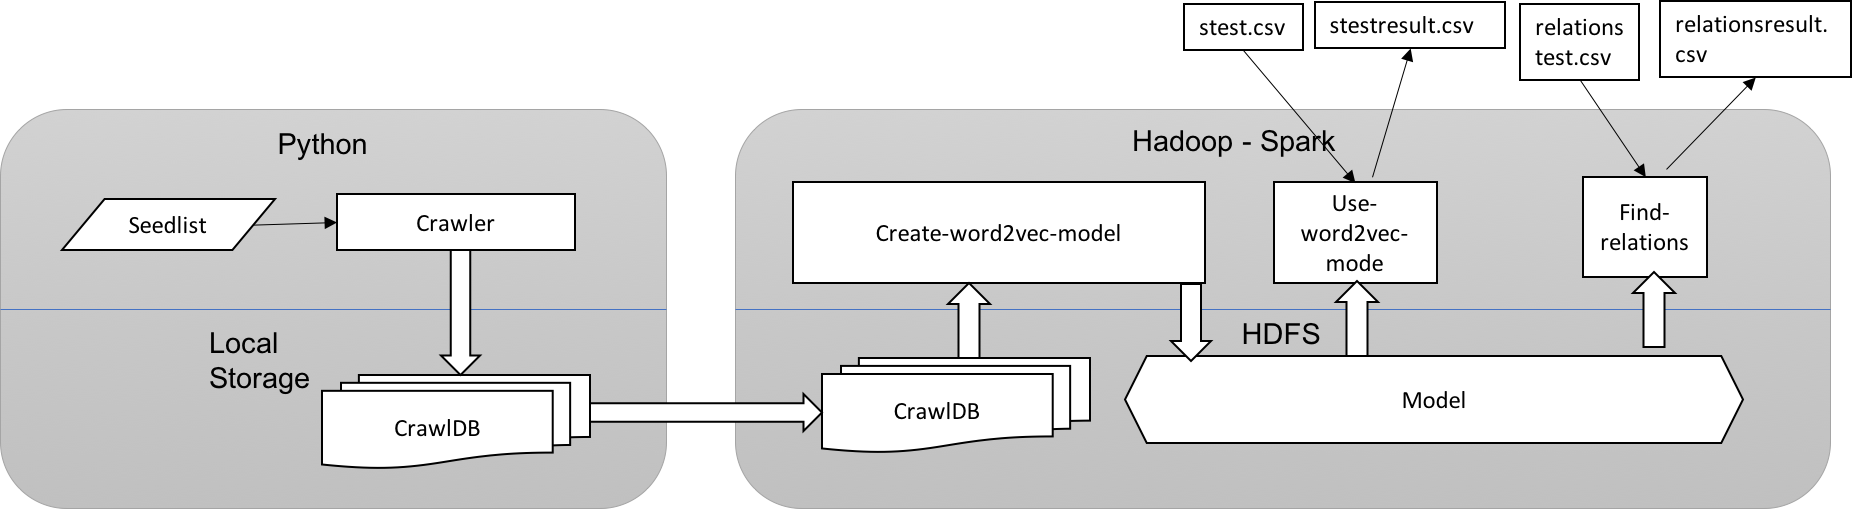
\includegraphics[width=\linewidth]{images/datapipeline.png}}
\caption{Data Pipeline.}
\label{fig:datapipeline}
\end{figure}

Figure \ref{fig:datapipeline} shows the overall data pipeline for the
project. The data pipeline has three important stages:
\begin{itemize}
\item Crawler: Crawler runs in batch mode on a standalone machine. It can
download wikipedia data as explained in section \ref{crawlersection}. Crawler
 creates CrawlDB which is a collection of text files. This crawler can be
 replaced or augmented with any web-crawler which can download or create the
 text files.

\item create-word2vec-model: This component is responsible for creating the
word2vec model for the text files in the CrawlDB. This model runs on Spark
and stores the model on HDFS. Section \ref{createmodelsection} describes this
 component in detail.

\item use-word2vec-model and find-relations: These two components use the
precreated word2vec model to find synonym of a word or find the relationships.
Section \ref{usemodel} describes these components in detail.
\end{itemize}

\subsection{Crawler} \label{crawlersection}
The Crawler component is useful to download the data from web. We implemented
 a simple crawler using Python which can deep traverse the wikipedia pages
 and download the text from it. In our crawler implementation, a user can
 specify the seed pages from wikipedia. User can also specify the maximum
 number of pages that are required to be downloaded. The crawler first
 downloads all the pages specified in the seedlist. It then extract the links
  from each wikipedia page and puts it in a queue which is internally
  maintained by the crawler. The crawler then downloads the the linked pages.
   Since this logic is implemented in recursive manner, the crawler can
   potentially download all the wikipedia pages which can be reached from the
   pages in the seedlist.

    We followed the seedlist based crawler approach so that we can retrieve
    domain specific web pages. A well chosen seedlist can fetch large number
    of relevant web pages.

 Figure \ref{fig:crawleralgo} is the flowchart of the crawler implementation.
\begin{figure}[htbp]
\centering
\fbox{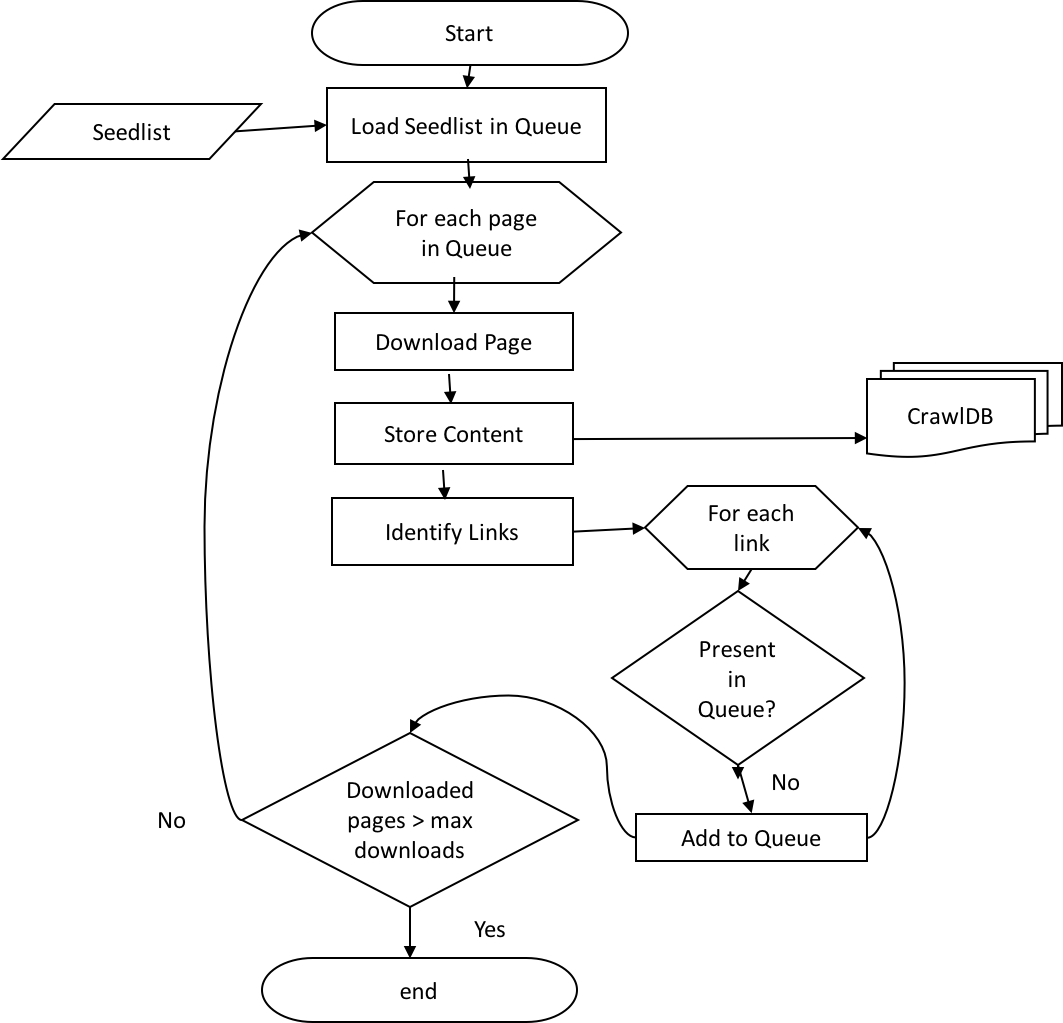
\includegraphics[width=\linewidth]{images/crawleralgo.png}}
\caption{Flowchart of crawler.}
\label{fig:crawleralgo}
\end{figure}

\subsection{Word2Vec Model Creation} \label{createmodelsection}


\subsection{Using the Word2Vec Model} \label{usemodel}




\section{Deployment} \label{deploymentsection}

The deployment on the cluster can be accomplished using 2 steps, assuming the cluster
is up and running
\begin{itemize}[noitemsep]
\item Step1: update hosts file \textit{ansible-word2vec/hosts} with the IP of the master. 
The first node on the cluster becomes the master node.
\item Step2: run the script  \textit{ansible-word2vec/run.sh}. This script will run the ansible 
playbooks to accomplish stage1 through stage4 of the deployment process.
\end{itemize}

\begin{figure}[htbp]
\centering
\fbox{\includegraphics[width=\linewidth]{images/deployment.png}}
\caption{Deployment stages.}
\label{fig:deploymentstages}
\end{figure}

Figure \ref{fig:deploymentstages} shows the deployment stages. The two steps
accomplish deployment in multiple stages as discussed in the sections below.

\subsection{Stage1} \label{deploymentstage1} 
As pre-requisite, we need to create a cluster with 1 or more nodes.
We created a 3 node cluster using Cloudmesh \cite{www-cloudmesh} command line interface(CLI). 
Cloudmesh\cite{www-cloudmesh} CLI allows you to orchestrate virtual machines(VM) in a 
cloud environment. For this project, we have used Chameleon and Jetstream cloud 
providers to orchestrate the VMs using cloudmesh\cite{www-cloudmesh} CLI. We can orchestrate a 3 node 
cluster using following CLI:

\begin{verbatim}
cm reset
pip uninstall cloudmesh_client
pip install -U cloudmesh_client
cm key add --ssh
cm refresh on
cm cluster define --count 3 \
	--image CC-Ubuntu14.04 --flavor m1.medium
cm hadoop define spark pig
cm hadoop sync
cm hadoop deploy
cm cluster cross_ssh
\end{verbatim}   

We are using Ubuntu14.04 image with m1.medium which comes with 2 CPU, 4GB
memory. Also, the nodes created are having hadoop and spark add-ons.
We can test the deployment by checking hdfs and spark-submit CLI work fine.
\begin{verbatim}
ssh cc@<cluster-ip>
sudo su - hadoop
hdfs
spark-submit
\end{verbatim}

At this stage our cluster is ready for further deployments.

\subsection{Stage2} \label{deploymentstage2}  
By default, cloudmesh installs spark 1.6 but our word2vec solution requires
spark 2.1. We need to upgrade spark on the cluster. In order to do so we can run 
\textit{install\_upgrade\_spark.yaml} ansible\cite{www-ansible} playbook. This will download and unpack spark2.1 
tar ball and further update the softlink to point to spark 2.1 folder.

\subsection{Stage3} \label{deploymentstage3} 
In this step, we upgrade the development libraries for python, and pip,
install python modules like wkipedia, request etc, download the code from git repo and
install it in \textit{/opt/word2vec} folder, set the folder permissions for the \textit{/opt/word2vec} folder
so that it can be executed by hadoop user. These steps can be achieved using 
\textit{word2vec\_setup.yaml} playbook. After completing this stage, we are ready for running
our word2vec solution on the cluster. 

\subsection{Stage4} \label{deploymentstage4} 
This stage primarily deals with submitting the jobs for various purpose. 
Before we submit the jobs, we need to make sure input folder are created on hadfs.
First, we run the crawler to download the training set and upload the data on hdfs.
Further we run various jobs to created model and find relations. Along with these jobs
we also run some monitoring jobs. The monitoring job queries spark metrics using 
\begin{verbatim}
http://${spark_master}:4040
\end{verbatim}

Stage4 steps can be accomplished using \textit{word2vec\_execute.yaml} playbook. 

At the end of stage4 we also fetch the execution results from the cluster along with the 
metrics of execution times at various stages. The output files are fetched into \textit{/tmp/word2vec\_results}
\begin{verbatim}
ls -1t /tmp/word2vec_results
jobs.csv
executors.csv
app.csv
stest.csv
relationstest.csv
stestresult.csv
relationsresult.csv
\end{verbatim}
Files \textit{jobs.csv, executors.csv, and app.csv} collect the execution time for various jobs. 
File \textit{relationsresult.csv} file collects the results for sample relations corresponding to
\textit{relationstest.csv}. Similarly \textit{stestresult.csv} collects the results corresponding to \textit{stest.csv}.

\subsection{Execution} \label{deploymentexecution}
\subsubsection{Cleanup}
We can execute the run from local system using  \textit{run.sh} located inside \textit{ansible-word2vec}. 
Run script executes all stages sequentially on the remote system. To rerun word2vec, run the cleanup 
playbook \textit{word2vec\_cleanup.yaml} located inside \textit{ansible-word2vec}.  Cleanup remove 
the spark 2.1 binary and the soft link, remove \textit{/opt/word2vec} folder as well as any temporary files created
during setup step.

\subsubsection{Page size}
The crawler downloads pages from wikipedia based on the config page count. To modify the page count, 
we can edit \textit{ansible-word2vec/setupvariables.yml} and set the \textit{max\_pages} to desired 
page size. The crawler downloads individual pages and then combines the pages into a single file
before submitting the spark jobs.

\subsubsection{Test Results}
Test results are downloaded to local machine in  \textit{/tmp/word2vec\_results} folder. Ansible execution
log is saved in \textit{/tmp/word2vec-logfile.txt}. The log gets appended each time you execute the run 
script.

\subsubsection{Troubleshooting}
\begin{enumerate}
\item If the installation \textit{run.sh} script fails in middle due to some reason, execute the cleanup script
before re-triggering run script again. The run script may fail due to variety of reasons like failed to shh,
hadoop not available etc
\item If the run script fails due to spark memory errors, you can modify the spark memory setting in
 \textit{code/config.properties} push the code to a git feature branch for example spark\_test. Modify
 \textit{word2vec\_setup.yaml} git section \textit{version=master} to point to spark\_test branch and 
 execute the run script.
 \item If hadoop goes into safe mode, goto the cluster namenode and execute the following
 \begin{verbatim}
 /opt/hadoop$ bin/hadoop dfsadmin -safemode leave
 \end{verbatim}
 This will remove the cluster from safe mode.
 \end{enumerate}
 
 
 



\section{Benchmarking} \label{benchmarking}
We used datasets of 2 different sizes to perform the benchmarking of the
application. Table \ref{tab:datasets} shows the details of the two datasets.
The CreateWord2VecModel spark application is most complex and time
consuming application. We used this application for the benchmarking. We
deployed the application on Chameleon cloud and Jetstream cloud. Table
\ref{tab:cloudconfig} shows the details for the cluster configurations on
Chameleon and Jetstream clouds.

\begin{table}[htbp]
\centering
\caption{\bf Dataset Used for Performance Measurement}
  \begin{tabular}{l|c|r}
    \hline
    Parameter & Dataset1 & Dataset2 \\
    Size of crawldb & 1.4MB & 7.4MB \\
    Count of files in crawldb & 100 & 500 \\
    Source & Wikipedia & Wikipedia \\
    \hline
  \end{tabular}
  \label{tab:datasets}
\end{table}


\begin{table}[htbp]
\centering
\caption{\bf Dataset Used for Performance Measurement}
  \begin{tabular}{ l | c | r }
    \hline
    Parameter & Chameleon Cluster & Jetstream Cluster \\
    Cluster name & cluster-005 & cluster-010 \\
    Nodes & 2 & 2 \\
    OS & Ubuntu 14.04 & Ubuntu 14.04 \\
    Flavor & m1.medium & m1.medium \\
    Secgroup & default & default \\
    Assign floating IP & True & True \\
    Cloud & chameleon & iujetstream \\
    \hline
  \end{tabular}
  \label{tab:cloudconfig}
\end{table}


Figure \ref{fig:compare147} shows the total time taken by CreateWord2Vec
application for Dataset1 on the Chameleon and Jetstream cloud environments.
\begin{figure}[htbp]
\centering
\fbox{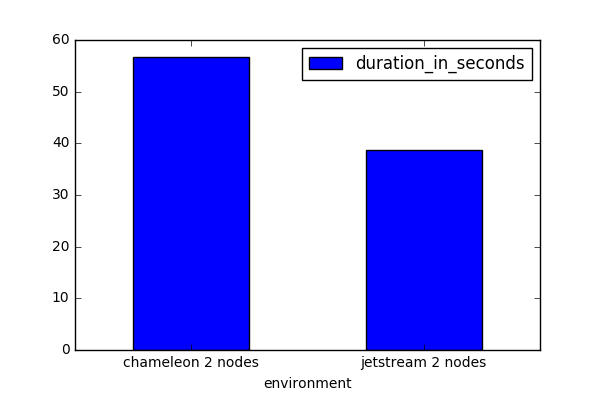
\includegraphics[width=\linewidth]{images/compare147.png}}
\caption{Time taken by CreateWord2Vec for Dataset1}
\label{fig:compare147}
\end{figure}

Figure \ref{fig:compare522} shows the total time taken by CreateWord2Vec
application for Dataset2 on the Chameleon and Jetstream cloud environments.
\begin{figure}[htbp]
\centering
\fbox{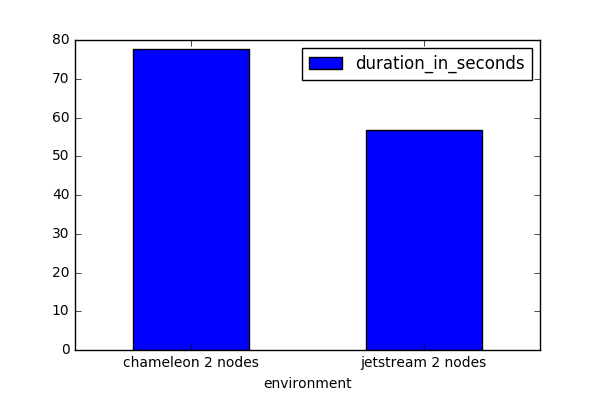
\includegraphics[width=\linewidth]{images/compare522.png}}
\caption{Time taken by CreateWord2Vec for Dataset2}
\label{fig:compare522}
\end{figure}

\subsection{Working with large dataset} \label{benchmarklargedatasets}
There are several configuration parameters added in the application to
fine tune the behavior of the spark applications. When working with larger
datasets, the spark applications can go out of memory. Following parameters
can be configured in the config.propertise to handle such situation.

\begin{verbatim}
spark_executor_memory = <memory given to executor>
spark_driver_memory = <memory given to driver>
max_result_size = <maximum result size>
\end{verbatim}



\section{Discussion}
The analysis of the results provided interesting insights.
Section \ref{appdiscussion} provides key insights on our experiments with
Word2Vec on Wikipedia data. Section \ref{deploymentdiscussion} provide key
insights on our experience of deployment and execution of Word2Vec
application on Chameleon and Jetstream cloud.
\subsection{Word2Vec app - key insights}
We trained the Word2Vec model with the wikipedia data of Indian Cricket team
members. We used \textit{List of India ODI cricketers} as seedlist and
downloaded 500 pages from Wikipedia. With this dataset, we observed that the
\textit{synonym} or correlated words were pretty accurate. Some interesting
examples and its explanation:

\textit{sachin -> tendulkar}

\textit{world -> cup}

Sachin Tendulkar \cite{www-wiki-sachin-tendulkar} is famous Indian cricket
player. Naturally, the words \textit{sachin} and \textit{tendulkar} are
highly correlated. The Word2Vec model was able to find this correlation.

Cricket World Cup \cite{www-wiki-world-cup} is one of the most viewed
sporting event and considered as the flagship event of the international
cricket. Hence the words \textit{world} and \textit{cup} are highly correlated
 in the context of cricket. The Word2Vec model was able to find this correlation.

However, when we tried to find the people relationships using the wikipedia
dataset, we could not get good accuracy. For example, \textit{Anjali Tendulkar}
 is wife of \textit{Sachin Tendulkar} while \textit{Dona Ganguly} is wife of
 \textit{Sourav Ganguly} who is another famous Indian Cricket player
 \cite{www-wiki-sourav}. When we provided the test record of

 \textit{sachin,anjali,sourav}

 we did not get good results.

 After observing the wikipedia data, we concluded that there is lot of
 literature  in wikipedia about the cricketers. However, there were very few
 mentions of their family members, coaches, schools etc. Due to this, we were
  not getting good results on the people relationships.

  To augment the Wikipedia data, we decided to crawl news data which provide
 large amount of articles containing people and their relationships. We
 implemented the news crawler as explained in the section
 \ref{newscrawlersection}. After downloading about 200 news articles of 20
 cricketers, our relationships discovery improved a lot. Some interesting
 examples are given below:
 \textit{sachin,anjali,sourav,dona}

 \textit{sachin,anjali,dhoni,sakshi}

 \textit{sachin,cricket,amitabh,hero}

 In first two examples, the Word2Vec model was able to identify the
 people-people relationships, while in third example, the Word2Vec model was
 able to identify the people-profession relationships.







 \label{appdiscussion}
\subsection{Deployment of Word2Vec app on Chameleon and JetStream cloud - key
insights}
Both Chameleon and Jetstream run on openstack and work seamlessly using
cloudmesh and ansible. There is a difference in the flavor for Chameleon and Jetstream,
where m1.medium on Chameleon is different than m1.medium on Jetstream. \label{deploymentdiscussion}

\section{Conclusion}

Using this project we conclude that we can use Word2Vev model on Wikipedia
and news data to find the relationships between the people.

We further conclude that Word2Vec based analytics can be performed on public
cloud systems like Chameleon cloud and Jetstream cloud. Our deployment
automation, which is implemented using Cloudmesh and Ansible technology
demonstrates the power of these technologies to achieve one touch deployment
and execution of applications across multiple clouds.

\section{Acknowledgement}

We acknowledge our professor Gregor von Laszewski and all associate instructors for helping us and guiding us throughout this project.

\section{Appendices}
Appendix A: Work Distribution
The co-authors of this report worked together on the design of the technical
solutions, implementation, testing and documentation. Below given is the work
 distribution
\begin{itemize}
\item Avadhoot Agasti
    \begin{itemize}
    \item Implementation of wiki crawler and news cralwer in Python.
    \item Implementation of CreateWord2VecModel in Spark.
    \item Implementation of UseWord2VecModel and FindRelations in Spark.
    \item Implementation of Python script MonitorSparkApp.
    \item Analyzing the Word2Vec model results.
    \item Testing of end to end flow on Chameleon cloud.
    \item Performance testing and bug fixing in the spark application.
    \item Writing related sections in this report.
    \end{itemize}

\item Abhishek Gupta
    \begin{itemize}
    \item Implementation of Ansible scripts for deployment of Spark 2.1 which
     is required for the spark application.
    \item Implementation of Ansible scripts for deployment.
    \item Implementing the changes in the spark applications to get it
    working on HDFS.
    \item Setting up and testing the end to end flow on Chameleon cloud.
    \item Setting up and testing the end to end flow on Jetstream cloud.
    \item Testing the crawler and Word2Vec applications for semantic
    correctness.
    \item Gathering the perfomance statistics for comparison.
    \item Writing related sections in this report.
    \end{itemize}
\end{itemize}

% Bibliography

\bibliography{references}

\end{document}
